%This is the last chapter 
%%=========================================
 \rhead{\itshape Cloud Computing}
\chapter{Cloud Computing}

\section{Introduction}
Il est communément admis que le concept de cloud computing a été initié par le géant d'Amazon en 2002. Le cybermarchand a ensuite investi dans un parc informatique pour pallier les surcharges de serveurs dédiées au commerce en ligne observées pendant les vacances. À cette époque, Internet comptait moins de 600 millions d'utilisateurs, mais l'utilisation du Web et les achats en ligne augmentaient. Malgré cette augmentation, les ressources informatiques d'Amazon sont restées peu utilisées une fois la période des fêtes terminée. Cette dernière a alors eu l'idée de louer ses capacités informatiques le reste de l'année à des clients pour stocker les données et utiliser les serveurs. Ces services étaient accessibles via Internet et avec une adaptation en temps réel des capacités de traitement, toutes facturées à la consommation. Cependant, ce n'est qu'en 2006 qu'Amazon s'est rendu compte qu'un nouveau mode de consommation des ordinateurs et d'Internet émergeait \cite{c1}.


Avant la naissance du terme cloud computing, utilisé par les informaticiens pour décrire l'immense nébuleuse du net, les services cloud étaient déjà utilisés comme webmail, stockage de données en ligne (photos, vidéos ...) ou partage d'informations sur les réseaux sociaux.


Dans les années 1990, un autre concept avait déjà préparé le terrain pour le Cloud Computing. Il s'agit de l'ASP (Application Service Provider) qui a permis au client de louer l'accès au logiciel installé sur les serveurs distants d'un fournisseur de services, sans installer le logiciel sur ses propres machines. Le Cloud Computing ajoute à cette offre la notion d'élasticité avec la possibilité d'ajouter de nouveaux utilisateurs et services d'un simple clic de souris \cite{c1}.


La virtualisation est un concept beaucoup plus ancien qui est à la base du cloud computing. La virtualisation est un ensemble de techniques matérielles ou logicielles utilisées pour exécuter plusieurs configurations informatiques (systèmes d'exploitation, applications, RAM, etc.) sur une seule machine physique pour former plusieurs machines virtuelles qui reproduisent le comportement des machines physiques. C'est le fait de formaliser une offre de services informatiques dématérialisés à la demande en direction des entreprises qui a été le moteur du développement du Cloud Computing en tant que tel.
\section{Définition du Cloud Computing}
Le cloud computing est le mot qui a fait le plus de buzz ces dernières années, vous le trouvez partout, feuilletez un magazine technologique ou visitez n'importe quel site ou blog de l'informatique, vous allez sûrement rencontrer une discussion sur le cloud computing, le seul problème est que non tout le monde s'accorde sur la définition du Cloud, si vous posez la question «Qu'est-ce que le Cloud Computing?» Accélérez les experts dans le domaine Vous aurez dix réponses différentes. Et le cloud est-il à la mode? ! Pour certains, ils disent que ce n'est qu'un concept marketing de vendre des produits classiques. En revanche, d'autres y voient l'avenir des applications et une rupture technologique majeure dans l'histoire de l'informatique, pour vous apporter un éclairage objectif nous vous proposons plusieurs définitions par différents acteurs du marché informatique.


En 2009, le NIST (National Institut of Standards and Technologie) a donné une définition du cloud computing largement adoptée et référencée. «Le Cloud Computing est l'ensemble des disciplines, technologies et modèles commerciaux utilisés pour fournir des capacités informatiques (logiciels, plates-formes, matériels) en tant que service à la demande».


Une deuxième définition est donnée en 2009 par l'Université de Californie à Berkeley qui considère que "le Cloud Computing désigne à la fois les applications fournies sur les services Internet et le matériel et les logiciels du système dans les centres de données qui fournissent ces services".



Ces deux définitions commencent à introduire des termes spécifiques au cloud, décrivant le cloud comme l'ensemble complet des phénomènes allant du faible niveau de matériel au haut niveau de service ou d'applications, ils introduisent également le concept de tout en tant que service référencé. Temps par XaaS (X = Logiciel ou Plateforme ou Matériel ...), dont une partie peut être livrée, mesurée et payable en tant que service \cite{c2}.

\section{Caractéristiques du cloud computing }
Il y a cinq propriétés qui caractérisent le cloud, nous appelons un service cloud lorsqu'il y a:
\subsection{Abstraction sur la localisation des données}
Le Cloud désigne un ordinateur où les données sont confisquées sans connaître leur localisation  géographique. L'application cloud se trouvant à San Francisco, Paris ou Pékin: cela fait peu de différences pour nous. Le mot «Cloud» fait principalement référence à cette abstraction sur le terrain. La métaphore est la suivante: les vrais clouds se déplacent perpétuellement autour de la terre, on ne sait pas les localiser, il en va de même pour le Cloud dont la position géographique des données est inconnue.


Certains acteurs du monde du Cloud jouent sur cette abstraction: ainsi Google entretient un certain mystère autour de la localisation de ses Datacenter. Il est donc impossible de savoir dans quel pays Google stocke vos données, ce qui peut être perturbant pour certains.


Le concept de déplacement perpétuel des clouds peut également avoir un sens avec le cloud : en effet, certains acteurs mettent en place des systèmes de déplacement et de réplication des données entre leurs Datacenters. Ces déplacements ont deux objectifs: disposer de plusieurs copies des données pour assurer leur conservation en cas de panne, et optimiser le remplissage des différents Datacenters, c'est-à-dire éviter les serveurs à moitié pleins. Ces mouvements étant automatiques, personne ne connaît l'emplacement des données, pas même les responsables des Datacenters.
\subsection{Souscription en ligne}
vous vous inscrivez via un formulaire, vous recevez un e-mail de confirmation, et le service peut être utilisé quelques secondes plusieurs tard. . . S'abonner en ligne semble naturel aujourd'hui, à l'heure du web. Mais il ne faut pas oublier qu'il existe encore un certain nombre de services qui ne peuvent pas être souscrits en ligne: les banques en ligne (à quelques exceptions près), l'assurance, etc. Cependant, ces services sont informatisés et ne nécessitent pas de rencontres physiques.
\subsection{Tarification « Freemium »}
Ce terme est la contraction des mots "Gratuit" et "Premium". Cela signifie qu'il existe une offre gratuite, parfois limitée dans le temps ou la capacité, ou offrant moins de fonctionnalités, et une offre payante pour les fonctionnalités avancées. L'offre payante est facturée en fonction des services disponibles ou en fonction de la capacité utilisée. Par exemple, la solution de stockage de fichiers DropBox de Cloud est gratuite pour 2 Go d'espace, puis devient payable au-delà.
\subsection{Accès depuis n'importe quel appareil}
Ordinateur, tablette, iPhone (Apple), Android (Google) ou Windows Phone (Microsoft). Le Cloud permet l'accès depuis n'importe quel appareil: à la maison, au travail, depuis le domicile d'un ami, depuis un cybercafé à l'étranger ... offre donc la certitude qu'il sera possible d'accéder à ses données où que vous soyez, à condition d'avoir une connexion à Internet et un navigateur Web. Cela peut être pratique en cas d'incident à l'étranger: il est astucieux d'avoir une copie de son passeport et de sa licence dans le Cloud pour anticiper les problèmes devant les voyageurs \cite{c3}.
\section{Techniques de virtuatisation}
Dans cette section nous presentons les concepts clé de la virtualisation.
\subsection{Définition}
La virtualisation a été la première pierre de l'ère du cloud computing, c'est l'ensemble des techniques et outils permettant de réaliser plusieurs systèmes d'exploitation sur une même machine physique pour offrir une meilleure utilisation des ressources, cette technologie vient répondre à certains problèmes tels que:
\begin{enumerate}
    \item \textbf{Sous-exploitation des serveurs physiques:} on estime que dans un Datacenter privé, le taux d'utilisation moyen est de 10\%. Cela passe à 35\% sur une architecture virtuelle.
\item \textbf{La croissance du nombre de serveurs physiques :}les ressources physiques d'un serveur seront partagées entre différents serveurs virtuels, ce qui permet de ne pas acheter plusieurs serveurs physiques. 
\item \textbf{Sécurité et fiabilité :}isoler les services sur différents serveurs dans les systèmes de virtualisation.

\end{enumerate}
\subsection{Virtualisation}
La virtualisation permet de coexister plusieurs systèmes d'exploitation complètement isolés sur un même hôte. On distingue plusieurs techniques de virtualisation à savoir: l'isolement, la para virtualisation, et la virtualisation complète.

\begin{enumerate}
    \item \textbf{L'isolation : }il est possible de diviser un système d'exploitation en plusieurs espaces mémoire ou plusieurs contextes. Chaque contexte est géré par le système d'exploitation hôte. Cette isolation permet d'exécuter plusieurs fois la même application pour ne s'exécuter qu'une seule fois par machine. Les programmes de chaque contexte ne peuvent communiquer qu'avec les processus et les ressources associés à leur contexte. L'isolement n'est lié qu'aux systèmes Linux.
\begin{figure}[H]
\centering
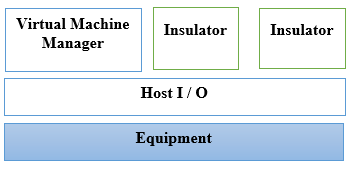
\includegraphics[scale=1]{chap1/fc1.png}
\caption{Architecture de l'isolation}
\label{fc1}
\end{figure}


\item \textbf{Para virtualisation (virtualisation de type 1):} c'est une technique de virtualisation qui présente à la machine invitée une interface logicielle similaire mais non identique au matériel réel. Ainsi, il permet aux systèmes d'exploitation invités d'interagir directement avec le système d'exploitation hôte et, par conséquent, ils seront conscients de la virtualisation.
\begin{figure}[H]
\centering
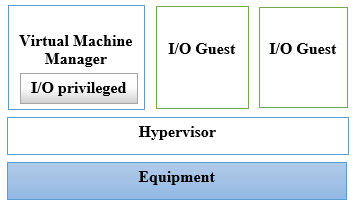
\includegraphics[scale=1]{chap1/fc2.png}
\caption{Architecture de la paravirtualisation}
\label{fc1}
\end{figure}


\item \textbf{Virtualisation complète (Virtualisation de type 2 virus):} il s'agit d'une technique de virtualisation qui crée un environnement entièrement virtuel. En utilisant ces techniques, le système d'exploitation invité n'interagit pas directement avec le système d'exploitation hôte et pense donc qu'il s'exécute sur une vraie machine physique. Cette technique de virtualisation permet uniquement la virtualisation des SE avec la même architecture matérielle que l'hôte.
\begin{figure}[H]
\centering
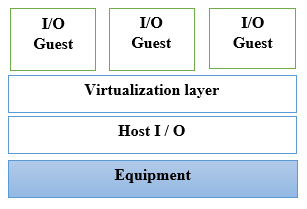
\includegraphics[scale=1]{chap1/fc3.png}
\caption{Architecture de la virtualisation complète}
\end{figure}
\end{enumerate}
\begin{table}[H]
\begin{tabular}{|l|c|c|c|}
\hline
                            & \multicolumn{1}{l|}{\textbf{isolation}} & \textbf{Paravirtualisation}                                                                                                                                                                       & \textbf{\begin{tabular}[c]{@{}c@{}}Virtualisation\\   complète\end{tabular}}                                                                                                                                          \\ \hline
\textbf{Types invités d'OS} & Linux                                   & \begin{tabular}[c]{@{}c@{}}Type différent mais avec \\ une architecture identique \\ (doit être adapté à la couche\\ de virtualisation -\textgreater conscient \\ d'être virtualisé)\end{tabular} & \begin{tabular}[c]{@{}c@{}}Type différent mais\\  avec une architecture \\ identique (non adapté à \\ la couche\\  de virtualisation-\textgreater \\ croit dialoguer \\ directement avec le \\ matériel)\end{tabular} \\ \hline
\textbf{Performance}        & ++ (Supplément faible)                  & \begin{tabular}[c]{@{}c@{}}+++ (Les invités SE \\ travaillent avec la \\ conscience d'être \\ virtualisés)\end{tabular}                                                                           & \begin{tabular}[c]{@{}c@{}}+ (L'unité centrale de \\ traitement, c'est-à-dire\\  le CPU, la RAM, \\ ainsi que la mémoire\\  de stockage,sont \\ directement accessibles \\ aux machines virtuelles)\end{tabular}      \\ \hline
\textbf{Simplicity}         & +++                                     & +                                                                                                                                                                                                 & ++                                                                                                                                                                                                                    \\ \hline
\textbf{Examples}           & OpenVZ                                  & Xen,HyperV                                                                                                                                                                                        & KVM, VirtualBox                                                                                                                                                                                                       \\ \hline
\end{tabular}
\end{table}

En conclusion, nous pouvons dire que:

\begin{itemize}
    \item 	L'isolement est considéré comme la solution la plus efficace, cependant, son inconvénient est qu'il est incomplet, donc le système d'exploitation doit être du même type Linux.
\item	La paravirtualisation suppose que le noyau de l'OS invité est légèrement modifié. Par conséquent, si le système n'a pas de fonctions dédiées à la paravirtualisation dans son noyau, cette technique devient inutilisable. L'objectif principal de cette technique est de fournir un accès presque identique aux ressources matérielles entre les systèmes hôte et invité.
\item La virtualisation complète  permet d'exécuter le système d'exploitation invité en mode natif sans modification. En revanche, cette solution est considéré comme la moins efficace car le système invité ne participe pas au processus de virtualisation et doit traverser la couche de virtualisation pour accéder aux ressources matérielles \cite{c4}.
\end{itemize}
\section{Services Cloud}
Les services proposés depuis le cloud peuvent être classés en trois grandes catégories, et les définitions choisies sont celles données par le NIST:
\begin{figure}[H]
\centering
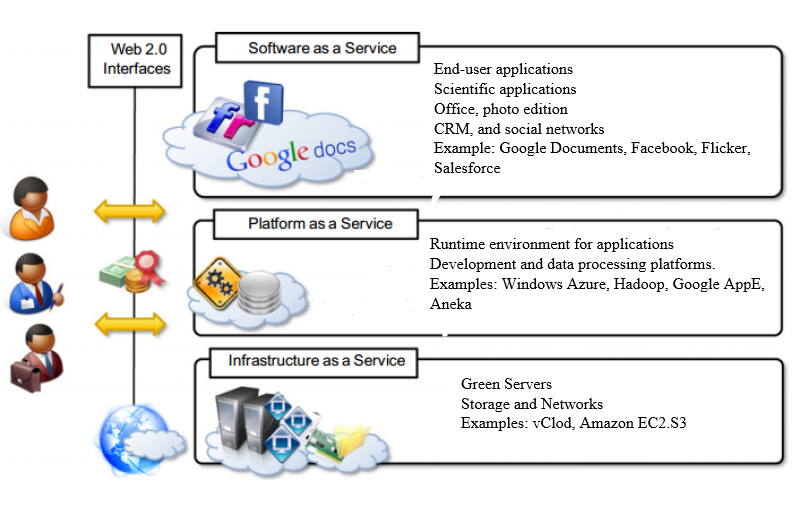
\includegraphics[scale=0.5]{chap1/fc4.png}
\caption{Modèle de référence du cloud computing}
\end{figure}

Les différentes couches de chaque catégorie sont presentés dans la figure \ref{fc5}

\subsection{Software as a Service (SaaS)}
Logiciel consommé en tant que service, le fournisseur de SaaS Cloud possède et gère l'ensemble de sa plateforme (du matériel au logiciel). Dans ce modèle, le client cloud utilise le logiciel mais ne s'occupe pas de la pile ci-dessous (plateforme d'application, matériel ...) ou de l'installation du logiciel Quelques exemples d'utilisation du modèle SaaS: E-mail, CRM (gestion de la relation client).Dans une solution SaaS, le contrôle des données est partagé entre le client (qui crée et utilise les données) et le fournisseur de cloud qui héberge, stocke, sécurise et sauvegarde les données).
\subsubsection{Les avantages}
\begin{itemize}
    \item Plus d'installation, plus de mises à jour (elles sont continués chez le fournisseur).
    \item Payez à l'utilisation.
    \item Testez facilement de nouveaux logiciels.
\end{itemize}
\subsubsection{Les inconvénients}
\begin{itemize}
    \item Limitation par définition du logiciel proposé.
    \item Aucun contrôle sur le stockage et la sécurisation des données associées
    \item La réactivité des applications Web n'est pas toujours idéale. Vers le logiciel \cite{c5}.

\end{itemize}
\subsection{Platform as a Service (PaaS)}
Une plate-forme sur laquelle les développeurs ou les éditeurs de logiciels peuvent déployer des applications. La pile (la plate-forme d'application, le système d'exploitation, le matériel, le réseau) est détenue et gérée par le fournisseur de services.
\subsubsection{Les avantages}
\begin{itemize}
    \item Le déploiement est automatisé (aucun logiciel supplémentaire à acheter ou à installer).

\end{itemize}
\subsubsection{Les inconvénients}
\begin{itemize}
    \item Limitez une ou deux technologies (par exemple Python ou Java pour Google AppEngine.NET pour Microsoft Azure, propriétaire de force.com).
    \item Aucun contrôle des machines virtuelles sous-jacentes.
    \item Convient uniquement aux applications Web.
\end{itemize}
\subsection{Infrastructure as a Service (IaaS)}
La plateforme sur laquelle les administrateurs informatiques pourront déployer une infrastructure (machine (s) virtuelle (s) + base d'applications + applications ..etc) Ce modèle, qui est une évolution des Datacenters virtualisés, permet au client de ne pas tenir compte du modèle physique (gestion des serveurs physiques, des éléments liés aux centres de données comme l'électricité, la climatisation, la sécurité physique). Dans ce modèle, le fournisseur contrôle le matériel et la couche de virtualisation. Au niveau des données, le contrôle est partagé au niveau de la machine virtuelle (qui est stockée et sauvegardée par le fournisseur de cloud IaaS).
\subsubsection{Les avantages}
\begin{itemize}
    \item Grande flexibilité.
    \item Contrôle complet du système (administration à distance par SSH ou Remote Desktop, RDP), qui permet d'installer tout type de logiciel d'entreprise.

\end{itemize}
\subsubsection{Les inconvénients}
\begin{itemize}
    \item Besoin d'administrateur système quant aux solutions de serveurs traditionnels sur site \cite{c5}.
\end{itemize}
\begin{figure}[H]
\centering
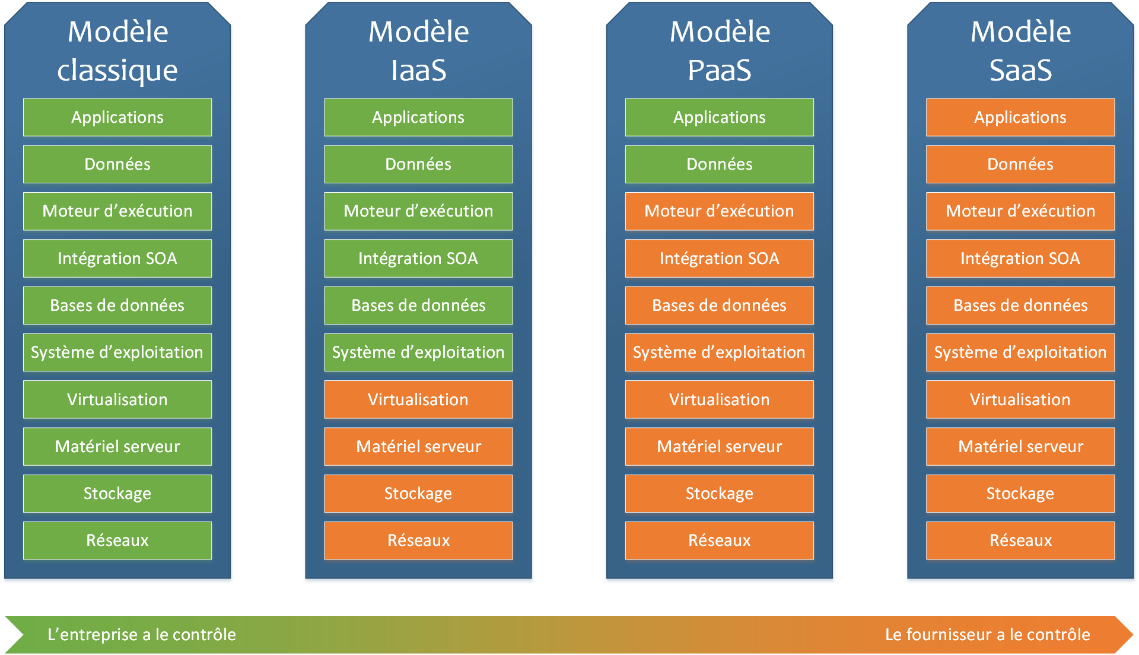
\includegraphics[scale=1.2]{chap1/fc5.png}
\caption{Différents types de services de cloud computing}
\label{fc5}
\end{figure}

\section{Modèles de cloud computing}
La figure \ref{fc6} montre les différents modèles de Cloud Computing, il en existe quatre modèles :
\subsection{Cloud privé}
Dans lequel toutes les ressources sont exclusivement mises à la disposition d'un seul client. Le cloud privé peut être géré par l'entreprise utilisatrice elle-même ou par un prestataire externe qui met à disposition de l'utilisateur un parc de machines adapté à la demande de l'utilisateur (Cloud privé virtuel). Notez qu'une même infrastructure peut accueillir plusieurs clouds privés virtuels appartenant à différents utilisateurs, chacun pouvant accéder à son cloud privé via son réseau.
\subsection{Cloud public}
Les utilisateurs ont accès aux services cloud via Internet public sans savoir exactement où leurs données sont hébergées ni où leur traitement est effectué. Les ressources informatiques et les bases de données de l'utilisateur peuvent être hébergées dans n'importe quel centre de données du fournisseur et peuvent passer d'un centre de données à un autre pour optimiser les capacités du fournisseur.

\begin{table}[H]
\caption{Principaux acteurs mondiaux du cloud public}
\begin{tabular}{|l|l|l|}
\hline
\multicolumn{1}{|c|}{\textbf{Iaas}}                                                            & \multicolumn{1}{c|}{\textbf{Paas}}                                                                   & \multicolumn{1}{c|}{\textbf{Saas}}                                                                                                                                                                                 \\ \hline
\begin{tabular}[c]{@{}l@{}}- Amazon-o\_res EC2 and AWS\\   - Microsoft-o\_re Azur\end{tabular} & \begin{tabular}[c]{@{}l@{}}- Microsoft-o\_re Azur\\   - Google-o\_re, Google App Engine\end{tabular} & \begin{tabular}[c]{@{}l@{}}- Google-o\_re,Google Apps\\ (messagerie et bureautique)\\   - SalesForce-CRM \\ (Gestion de la relation client)\\   - Microsoft-o\_re,o\_ce 365\\  (outils collaboratifs)\end{tabular} \\ \hline
\end{tabular}
\end{table}

\subsection{Hybride cloud}
Ils combinent infrastructure et cloud privé et public. Certaines données ou infrastructures sont gérées en interne par l'entreprise, dans ses locaux ou chez un fournisseur et communiquent avec les ressources Cloud. Le cloud hybride permet de différencier les lieux de traitement des données selon qu'elles sont stratégiques ou non: les données sensibles peuvent alors être traitées au sein des murs de l'entreprise tandis que les autres seront traitées par un cloud public plus rentable, plus efficace. Le cloud public peut également être une solution pour lisser un pic d'activité lorsque les capacités de l'entreprise sont obsolètes.
\subsection{Cloud communautaire}
Permettant à plusieurs entreprises où organisations de partager des ressources en mode Cloud, qui sont alors exclusivement dédiées à ces organisations. Le Cloud communautaire peut être géré par des organisations membres ou par un fournisseur externe. Le cloud communautaire peut également permettre à plusieurs utilisateurs de construire un cloud aux caractéristiques d'un cloud privé en termes de sécurité et de ressources dédiées, à moindre coût et avec une garantie d'indépendance vis-à-vis d'un prestataire de services de cloud public \cite{c1}.

\begin{figure}[H]
\centering
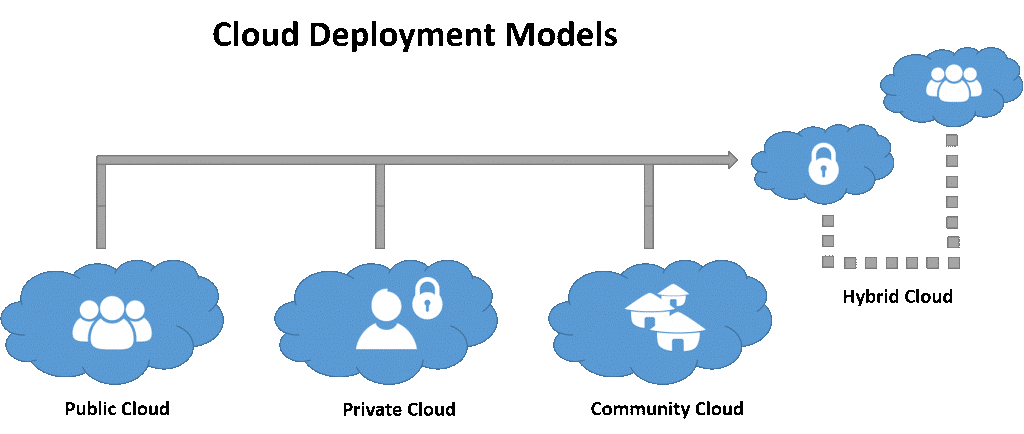
\includegraphics[scale=0.6]{chap1/fc6.png}
\caption{Modèles de déploiement cloud}
\label{fc6}
\end{figure}


\section{Avantages et inconvénients du Cloud Computing}
Le Cloud Computing représente la révolution dans l’informatique dans ces dernières années, ce paradigme-là arrive avec des avantages qui peuvent corriger les limites des autres technologies existées. Dans cette section, nous allons présenter quelques points forts de ce paradigme. Lorsqu’on parle d’un nouveau paradigme, les chercheurs ou les clients peuvent rencontrer toujours quelques limites \cite{c87}. Les avantages et les limites de ce paradigme seront présentés comme suit :
\begin{itemize}
    \item \textbf{Flexibilité :} le Cloud utilise multi-locataire pour ces ressources au cours de l’exécution, une application peut utiliser plusieurs ressources. Cela offre une possibilité de demander d’autres ressources s’il est besoins \cite{c87}.
    \item \textbf{Optimisation des coûts :} réduction des effectifs informatiques et fixation du prix en fonction de la durée d’utilisation des ressources informatiques sans investissement initiale lourd.
    \item \textbf{Évolutivité :} ça fait référence à un utilisateur Cloud (entreprise) qui peut utiliser d’énormes calculs de données dans un temps spécifique. A la fin du processus, le système peut retourner aux normes, tous sans nécessiter ces serveurs lourds \cite{c87}.
    \item \textbf{Portabilité :} les organisations peuvent utiliser leurs puissances informatiques partout où les utilisateurs peuvent avoir un accès dans n’importe quelle localisation géographique \cite{c87}.
    \item \textbf{Sécurité :} dans le Cloud, les fournisseurs utilisent des stratégies afin de garantir la vie privée de chaque utilisateur par : la réplication des données, plan de reprise d’activité, etc.
    \item \textbf{Simplicité d’utilisation :} le Cloud offre des applications et des services installés et faciles à utiliser à travers des pages web.
\end{itemize}


Comme nous avons mentionné, chaque nouvelle technologie arrivée porte des avantages et malheureusement suivi par quelques limites rencontrées par des utilisateurs du Cloud. Ces limites sont présentées comme suit :

\begin{itemize}
    \item \textbf{La gestion d’énergie :} afin de définir un plan d’utilisation des ressources, le fournisseur doit définir une stratégie pour la gestion d’énergie (consommation d’électricité) \cite{c87}
\item \textbf{Confidentialité et sécurité :} dans n’importe quelle technologie, la sécurité pose toujours des problèmes. Le problème concerne les attaques lors des opérations du transfert de données. Dans le cloud, ce problème est posé dans les cas des cloud publiques \cite{c87}.
\item \textbf{Gestion de ressources :} ce problème représente toujours les limites de chaque technologie. A cause de la nature multidimensionnelle des machines virtuelles, la gestion des ressources sera compliquée .
\item \textbf{Dépendance :} en cas ou l’entreprise (ou client final) souhaite des fonctionnalités très spécifiques, il est peut être difficile de convaincre le fournisseur de proposer ces fonctionnalités. Le client final doit choisir un fournisseur en qu’il a la confiance.
\item \textbf{Migration vers une autre offre difficile :} il n’existe pas pour l’instant un standard entre les différents acteurs du domaine, donc, le risque d’incompatibilité du transfert de données.

\end{itemize}

\section{Edge computing}
L’edge computing se définit comme une architecture informatique destinée aux environnements IoT, dans laquelle les ressources informatiques, la capacité de stockage et la puissance de calcul sont maintenues au plus près des équipements terminaux et des capteurs qui génèrent les données. Le concept représente ainsi une alternative aux solutions de Cloud ordinaires avec des serveurs centralisés.

Le mot « edge » vient de l’anglais et signifie bord ou périphérie. Ce terme fait allusion au fait que le traitement des données ne se fait plus dans le Cloud, mais il est décentralisé, en périphérie du réseau. L’edge computing peut ainsi offrir une option que le Cloud n’est pas capable de proposer, à savoir des serveurs capables d’interpréter sans délai les données de masse générées par des usines, des réseaux de distributions ou des systèmes de circulation « intelligents », et de prendre immédiatement les mesures nécessaires en cas d’incidents.
\subsection{Fondamentaux de l’edge computing}
L’edge computing est une nouvelle forme d’architecture pour les environnements IoT bien qu’elle n’ait pas directement recours à de nouveaux composants de réseau. Au contraire, elle s’appuie sur d’anciennes technologies dans un format compact, mais employées sous une nouvelle dénomination. Voici un aperçu des éléments de base de l’edge computing.
\subsubsection{Edge}dans le jargon informatique, le mot « edge » désigne la périphérie du réseau. Quant à savoir quels seront les éléments implantés en périphérie du réseau, cela dépendra de la configuration mise en place. Dans des réseaux de télécommunication, ce sera par exemple un téléphone portable qui représentera la périphérie du réseau ; et dans un système de voitures autonomes interconnectées, chaque véhicule. On parle dans ce cas d’un edge device.
\subsubsection{Edge device}on entend par edge device tout appareil situé en périphérie de réseau, et qui génère des données. Les sources de données possibles sont par exemple des capteurs, des machines, des véhicules ou tous les autres appareils intelligents dans un environnement IoT, comme des lave-linge, des détecteurs d’incendie, des ampoules ou des thermostats pour radiateur.
\subsubsection{La passerelle Edge} la passerelle Edge est une instance de calcul implantée à la transition entre deux réseaux. Dans des environnements IoT, les passerelles Edge sont utilisées comme nœuds entre l’Internet des objets et le réseau central. On a aussi de puissants routeurs, capables de supporter de fortes puissances de calcul pour assurer le traitement des données de l’IoT. Pour ce faire, les passerelles Edge disposent de diverses interfaces permettant de transférer les données soit par câble, soit par radio, et de standards de communication, comme l’Ethernet, le Wifi, le Bluetooth, la téléphonie 3G, LTE, Zigbee, Z-Wave, CAN-Bus, Modbus, BACnet ou SCADA.
\subsection{Edge computing et Fog computing}
L’approche visant à étendre le Cloud autour des instances de calcul n’est pas une nouveauté. En 2014 déjà, le groupe américain Cisco a créé le terme marketing, baptisé « fog computing». Ce concept est basé sur un traitement décentralisé des données dans ce qu’on appelle des « nœuds fogs ». Les nœuds fog représentent de mini-centres de calcul positionnés en amont du Cloud, constituant une couche intermédiaire dans le réseau (on parle de « couche fog »). Les données générées dans des environnements IoT ne sont donc pas directement envoyées dans le Cloud. Elles sont d’abord collectées dans des Fog Notes, où elles sont interprétées avant d’être sélectionnées pour d’autres formes de traitement.

L’edge computing est aujourd’hui considéré comme faisant partie du fog computing, où les ressources informatiques, comme la puissance de calcul et la capacité de stockage sont rapprochées au mieux des équipements IoT, en périphérie du réseau. Dans des architectures de fog computing, le traitement des données se fait d’abord au niveau de la couche fog, tandis que dans des concepts d’edge computing, il est exécuté au niveau de puissants routeurs IoT, et même parfois directement sur les appareils ou sur les capteurs. On peut parfaitement envisager une combinaison des deux concepts. Le graphique ci-dessous montre une telle architecture avec une couche Cloud, fog et edge.
\subsection{Domaines d’application pour les architectures d’edge computing}
Les domaines d’application pour l’edge computing viennent généralement de l’environnement IoT, et représentent des projets d’avenir au même titre que le concept d’une architecture Cloud décentralisée. Un facteur de croissance important de la technologie de l’edge computing est le besoin croissant de systèmes de communication fonctionnant en temps réel. Le traitement décentralisé des données est une technologie clé pour les projets suivants :

\begin{itemize}
    \item[*] La communication de véhicule à véhicule
     \item[*]Le réseau électrique intelligent
      \item[*]Le Smart Factory
\end{itemize}


Un véhicule connecté sera, à l’avenir, bien plus qu’un véhicule équipé d’une connexion Internet. L’avenir de la mobilité permettra la mise en place de systèmes d’avertissement gérés par le Cloud, permettant une communication de véhicule à véhicule, voire des moyens de transport complètement autonomes dans leurs déplacements. La condition est cependant que l’on puisse disposer d’une infrastructure permettant d’échanger en temps réel des données entre les véhicules et les différents points de communication tout au long de l’itinéraire.


Le réseau électrique de l’avenir sera lui aussi adaptatif, capable de s’auto-réguler automatiquement en fonction des besoins grâce à des systèmes de gestion d’énergie décentralisés. Dans le cadre de la transition énergétique, le réseau électrique intelligent représentera une technologie clé. En effet, la conversion vers des énergies renouvelables impose de nouveaux défis aux réseaux d’électricité. Au lieu d’avoir quelques gros producteurs centralisés, on aura de nombreux petits producteurs d’énergie décentralisés, avec des dispositifs de stockage qui devront être connectés avec les consommateurs. Certains d’entre eux seront eux-mêmes producteurs d’énergie, notamment grâce aux panneaux solaires. Les réseaux intelligents ne se contentent plus de transporter le courant électrique : ils délivrent également des données applicables à sa production, son stockage et sa consommation. Ceci permet à chacun de réagir en temps réel à la moindre modification. L’objectif est de maintenir la stabilité des réseaux électriques malgré leur complexité croissante, et d’assurer une meilleure efficacité grâce à une compensation intelligente des charges. Pour pouvoir saisir, sauvegarder et traiter dans les meilleurs délais toutes ces données générées, nous avons besoin de nouveaux concepts de Cloud, comme l’edge computing et le fog computing.


On entend par Smart Factory (usine du futur) des sites de production et des systèmes de logistique qui s'organisent eux-mêmes. Dans l’idéal, on n’a aucune intervention humaine dans de tels concepts. Une usine intelligente est un système interconnecté d’appareils, de machines et de capteurs qui communiquent entre eux par Internet pour mener à terme des processus de fabrication. Le système de communication Smart Factory inclut le produit fini dans son système et peut donc réagir automatiquement face à des demandes de devis. Grâce à des systèmes d’intelligence artificielle et à un apprentissage autonome, on a des processus de maintenance qui optimisent la production. Ceci demande une infrastructure informatique capable de traiter sans délai de gros volumes de données, et de réagir rapidement à des imprévus. Les systèmes de Cloud traditionnels échouent pour des raisons de latence. Les architectures d’edge computing et de fog computing peuvent résoudre ce problème grâce à un traitement des données partagé.

\subsection{Avantages et inconvénients de l'edge computing}
Le tableau ci-dessous présente les avantages et les inconvénients d’une architecture d’edge computing, comparée à un environnement Cloud traditionnel \cite{mur1994edge}.

% Please add the following required packages to your document preamble:
% \usepackage[normalem]{ulem}
% \useunder{\uline}{\ul}{}
\begin{table}[H]
\begin{tabular}{|l|l|}
\hline
\multicolumn{1}{|c|}{\textbf{Avantages}}                                                                                                                                                                                                                                                                                                                            & \multicolumn{1}{c|}{\textbf{Inconvénients}}                                                                                                                                                                                                                                                                                                                                                                            \\ \hline
\begin{tabular}[c]{@{}l@{}}Traitement des données en temps réel : dans les \\ architectures d’edge computing, les unités de \\ calcul sont rapprochées au mieux des sources \\ de données, favorisant une communication en\\  temps réel. On évite ainsi le problème récurrent \\ de latence rencontré avec les solutions de Cloud \\ plus classiques.\end{tabular} & \begin{tabular}[c]{@{}l@{}}Des structures de réseau plus complexes : un \\ système de répartition est bien plus compliqué \\ qu’une architecture Cloud centralisée. Un \\ environnement edge computing est un ensemble \\ hétérogène de plusieurs composants de réseau, \\ venant en partie de divers fabricants, et qui \\ communiquent les uns avec les autres grâce à un \\ grand nombre d’interfaces.\end{tabular} \\ \hline
\begin{tabular}[c]{@{}l@{}}Débit utile réduit : l’edge computing privilégie un \\ traitement des données en local au niveau de \\ passerelles Edge. Seules les données qui ne \\ peuvent pas être traitées localement, ou qui \\ doivent être mises en lignes, sont téléchargées \\ dans le Cloud.\end{tabular}                                                     & \begin{tabular}[c]{@{}l@{}}Les frais d’acquisition pour du matériel Edge : les \\ architectures de Cloud se distinguent avant tout \\ par le fait qu’il y a beaucoup moins d’équipement \\ matériel à installer localement. On perd cet avantage\\  si on opte pour des systèmes à répartition.\end{tabular}                                                                                                           \\ \hline
\begin{tabular}[c]{@{}l@{}}La sécurité des données : avec une solution \\ d’edge computing, la majeure partie des \\ données reste dans le réseau local. Dans\\  une telle configuration, les entreprises \\ auront plus de facilité à se conformer aux \\ exigences de conformité.\end{tabular}                                                                    & \begin{tabular}[c]{@{}l@{}}Un niveau de maintenance plus élevé : un système \\ décentralisé, composé de plusieurs nœuds de calcul,\\  nécessite plus d’entretien et d’administration qu’un \\ centre de données.\end{tabular}                                                                                                                                                                                          \\ \hline
\end{tabular}
\end{table}
\section{Conclusion}
Dans ce chapitre, nous avons donné un aperçu sur la technologie du Cloud Computing. Comme nous avons vu que le Cloud pense à résoudre les problèmes posés dans les autres technologies. De plus, le Cloud représente une révolution car il offre des services de plusieurs types. Grâce aux bénéfices offerts par le fournisseur du Cloud, les utilisateurs finaux et les entreprises trouvent que le Cloud est un bon choix pour l’utilisation de ces services. 


Avec toutes ces solutions et les avantages produits dans le Cloud, il existe toujours des limites que nous avons détaillés dans ce chapitre. On a parlé aussi de la sécurité par ce qu’elle représente la vie privée des clients. Mais tout le monde maintenant utilise le Cloud Computing que ce soit personnel ou partagé avec les membres des équipes de la société.


Dans le prochain chapitre nous allons présenté un état de l’art sur les approches de l’Internet des objets  dans le smart house.
